\section{DElight Daylighting Calculations}\label{delight-daylighting-calculations}

The Daylighting:DELight series of input objects provide an alternative daylighting model.~ The DElight method of analyzing daylighting applies to both simple apertures (i.e., windows and skylights) and complex fenestration systems that include geometrically complicated shading (e.g., roof monitors) and/or optically complicated glazings (e.g., prismatic or holographic glass).~ The DElight daylighting calculation methods are derived from the daylighting calculations in DOE-2.1E (as are the models accessed with Daylighting:Controls input object), and Superlite, with several key modifications.~ The engineering documentation included here focuses on the details of these differences from methods documented elsewhere.~ For the details of the heritage calculations, refer to the section in this documentation entitled ``Daylighting Calculations'' and to {[}Winkelmann, 1983{]}, {[}Winkelmann and Selkowitz, 1985{]}, and~ {[}Modest, 1982{]}.

For each point in time, DElight calculates the interior daylighting illuminance at user specified reference points and then determines how much the electric lighting can be reduced while still achieving a combined daylighting and electric lighting illuminance target.~ The daylight illuminance level in a zone depends on many factors, including exterior light sources; location, size, and visible light transmittance of simple and complex fenestration systems; reflectance of interior surfaces; and location of reference points. The subsequent reduction of electric lighting depends on daylight illuminance level, design illuminance setpoint, fraction of zone controlled by reference point, and type of lighting control.

The DElight daylighting calculation has three main steps:

1.~~~~\emph{Daylight Factor Calculation:}~ Daylight factors, which are ratios of interior illuminance to exterior horizontal illuminance, are pre-calculated and stored for later use. The user spcifies the coordinates of one or more reference points in each daylit zone. DElight first calculates the contribution of light transmitted through all simple and complex fenestration systems in the zone to the illuminance at each reference point, and to the luminance at subdivided nodal patches of interior surfaces, for a given exterior luminous environment (including sky, sun, and exterior reflecting surfaces).~ The effect of inter-reflection of this initial light between interior reflecting surfaces is then calculated, resulting in a final total illuminance at each reference point.~ This total illuminace is then divided by the exterior horizontal illuminance for the given exterior environment to give a daylight factor.~ Daylight factors are calculated for each reference point, for a set of sun positions and sky conditions that are representative of the building location.

2.~~~~\emph{Time-Step Interior Daylighting Calculation}:~ A daylighting calculation is performed for each heat-balance time step when the sun is up. In this calculation the illuminance at the reference points in each zone is found by interpolating the stored daylight factors using the current time step sun position and sky condition, then multiplying by the exterior horizontal illuminance.

3.~~~~\emph{Electric Lighting Control Calculation}:~ The electric lighting control system is simulated to determine the proportion of lighting energy needed to make up the difference between the daylighting illuminance level at the given time step, and the design illuminance level. Finally, the zone lighting electric reduction factor is passed to the thermal calculation, which uses this factor to reduce the heat gain from lights.

\subsection{DElight Daylight Factor Calculation Differences from EnergyPlus Detailed Methods}\label{delight-daylight-factor-calculation-differences-from-energyplus-detailed-methods}

\begin{itemize}
\item
  \emph{Initial Interior Illuminance/Luminance Calculation:}~ DElight calculates the total initial contribution of light transmitted through all simple fenestration systems (i.e., windows and skylights) in the zone to the illuminance at each reference point, and to the luminance at each gridded nodal patch of interior surfaces.~ This differs from the models behind the ``Daylighting:Controls'' object (henceforth referred to as ``EnergyPlus Detailed'') in two ways. The first is that EnergyPlus Detailed calculates initial illuminace values at reference points for each pair of reference point and aperture (window/skylight) in the zone, whereas DElight calculates the total contribution from all apertures to each reference point.~ The second difference from EnergyPlus Detailed is that the initial luminance of interior surface nodal patches is calculated to support the inter-reflection calculation described below.~ This calculation uses the same formula as EnergyPlus Detailed modified for arbitrarily oriented surfaces (i.e., non-horizontal), and to calculate luminance rather than illuminance.~ Note however, DElight does not account for interior surface obstructions (e.g., partitions) in this initial interior illuminance/luminance distribution.~ The EnergyPlus Detailed method does account for interior surface obstruction of initial illuminance distribution on reference points.
\item
  \emph{Reference Points:}~ DElight allows up to 100 reference points to be arbitrarily positioned with a daylighting zone.~ At this time all reference points are assumed to be oriented on a horizontal virtual surface ``facing'' toward the zenith and ``seeing'' the hemisphere above the horizontal plane.
\item
  \emph{Complex Fenestration System Calculation:}~ DElight calculates the contribution to the initial interior illuminance at each reference point, and to the luminance at each gridded nodal patch of interior surfaces, of the light transmitted by complex fenestration systems (CFS).~ The analysis of a CFS within DElight is based on the characterization of the system using bi-directional transmittance distribution functions (BTDF), which must be either pre-calculated (e.g., using ray-tracing techniques) or pre-measured, prior to analysis by DElight.~ A BTDF is a set of data for a given CFS, which gives the ratios of incident to transmitted light for a range of incoming and outgoing directions.~ As illustrated in Figure~\ref{fig:bi-directional-transmittance-data.}, a BTDF can be thought of as collapsing a CFS to a ``black box'' that is represented geometrically as a flat two-dimensional light-transmitting surface that will be treated as an aperture surface in the daylit zone description. For each incoming direction across the exterior hemisphere of the CFS, varying portions of that light are transmitted at multiple outgoing directions across the interior hemisphere of the CFS.~ The two-dimensional CFS ``surface'' and directional hemispheres are ``abstract'' in that they may not literally correspond to actual CFS component geometric details.
\end{itemize}

\begin{figure}[hbtp] % fig 62
\centering
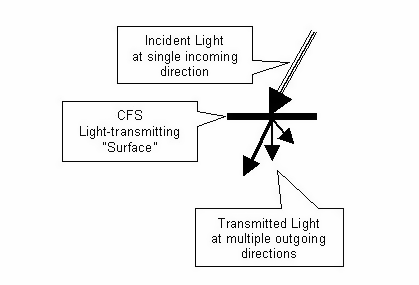
\includegraphics[width=0.9\textwidth, height=0.9\textheight, keepaspectratio=true]{media/image827.png}
\caption{Bi-Directional Transmittance Data. \protect \label{fig:bi-directional-transmittance-data.}}
\end{figure}

The pre-calculated or pre-measured BTDF for a CFS is independent of its final position and orientation within a building.~ Once a specific instance of a CFS aperture has been positioned within a building, the incident light from all exterior sources across the CFS exterior hemisphere can be integrated over all incident directions for each relevant transmitted direction to determine the light transmitted by the CFS surface in that direction. The light transmitted by the CFS aperture is then distributed to surfaces in the zone according to its non-uniform directionality.~ The algorithms for this BTDF treatment of CFS in DElight are still under development, and are subject to change in the future.

\begin{itemize}
\tightlist
\item
  \emph{Inter-reflected Interior Illuminance/Luminance Calculation:}~ The effect of inter-reflection of the initial interior illuminance/luminance between interior reflecting surfaces is calculated using a radiosity method derived from Superlite {[}Modest, 1982{]}.~ This method subdivides each reflecting surface in the zone into nodal patches and uses view factors between all nodal patch pairs in an iterative calculation of the total contribution of reflected light within the zone.~ This method replaces the split-flux method used in EnergyPlus Detailed, resulting in a more accurate calculation of the varied distribution of inter-reflected light throughout the zone.~ The ability to input up to 100 reference points supports a more complete assessment of this distribution.~ Also, the radiosity method explicitly accounts for interior obstructions between pairs of nodal patches.~ The split-flux method used in the EnergyPlus Detailed approach only implicitly accounts for interior surfaces by including their reflectance and surface area in the zone average surface reflectance calculations.
\end{itemize}

\subsection{DElight Time-Step Interior Daylighting Calculation Differences from EnergyPlus Detailed Methods}\label{delight-time-step-interior-daylighting-calculation-differences-from-energyplus-detailed-methods}

\begin{itemize}
\item
  \emph{Interior Illuminance Calculation:}~ As discussed above, DElight only calculates daylight factors for the total contribution from all windows/skylights and CFS to each defined reference point.~ Thus DElight does not support dynamic control of fenestration shading during the subsequent time-step calculations, as does EnergyPlus Detailed.
\item
  \emph{Visual Quality:}~ DElight does not currently calculate a measure of visual quality such as glare due to daylighting.~ DElight does calculate luminance on nodal patches of all interior, reflecting surfaces.~ A variety of visual quality metrics could be calculated from these data in future implementations.
\item
  \emph{Electric Lighting Control Calculation:}~ Up to 100 reference points can be defined within a DElight daylighting zone.~ One or more of these reference points must be included in the control of the electric lighting system in the zone.~ Each reference point input includes the fraction of the zone controlled by that point.~ Values of 0.0 are valid, which allows the definition of reference points for which interior illuminance levels are calculated, but which do not control the electric lighting.~ Any non-zero fraction is thus the equivalent of a relative weighting given to that reference point's influence on the overall electric lighting control.~ The sum of all fractions for defined reference points must less than or equal to 1.0 for this relative weighting to make physical sense.~ If the sum is less than 1.0, the remaining fraction is assumed to have no lighting control.
\end{itemize}

\subsection{References}\label{references-017}

Modest, M. 1982. A General Model for the Calculation of Daylighting in Interior Spaces, Energy and Buildings 5, 66-79, and Lawrence Berkeley Laboratory report no. LBL-12599A.

Winkelmann, F.C. 1983. Daylighting Calculation in DOE-2\emph{.} Lawrence Berkeley Laboratory report no. LBL-11353, January 1983.

Winkelmann, F.C. and S. Selkowitz. 1985. Daylighting Simulation in the DOE-2 Building Energy Analysis Program\emph{.} Energy and Buildings 8, 271-286.
